\documentclass{standalone}
\usepackage{tkz-fct}
\usepackage{tkz-euclide}
\usepackage{color}
\renewcommand*\familydefault{\sfdefault}
\usepackage{sansmath}
\sansmath
\definecolor{gray75}{gray}{0.75}
\begin{document}
 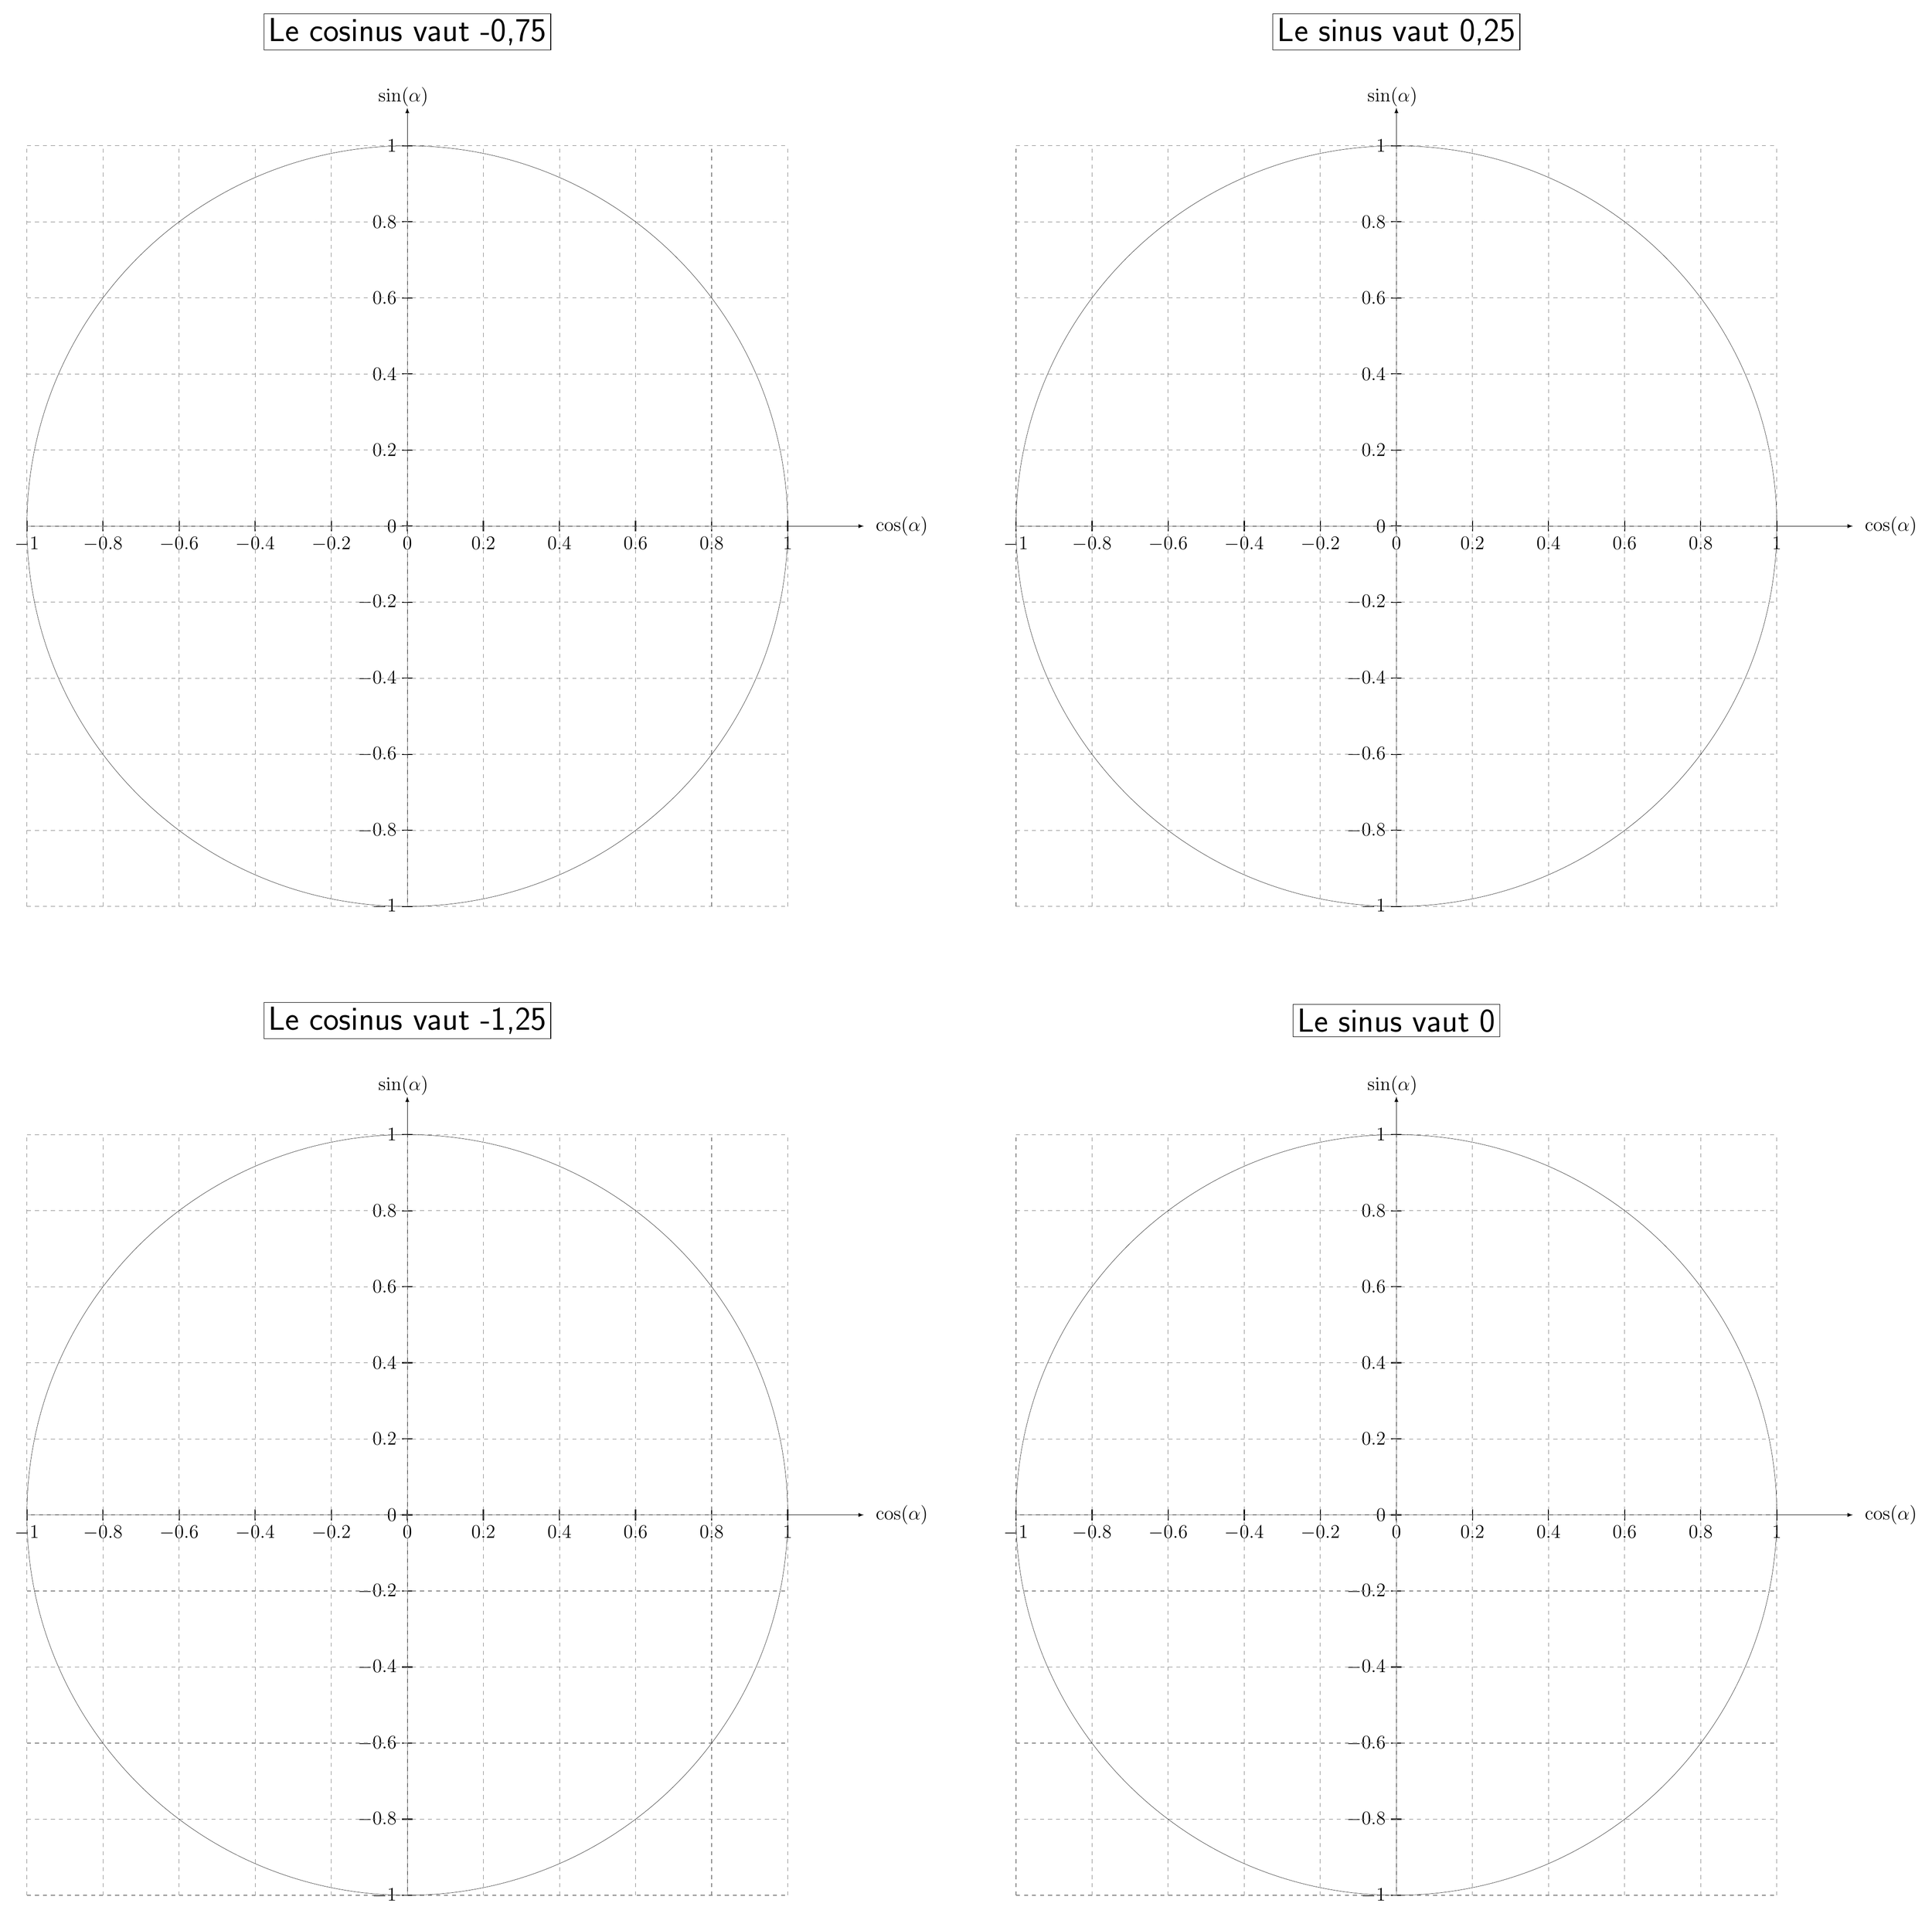
\begin{tikzpicture}[scale=2]
   \tkzInit[xmax=1.,ymax=1.,xmin=-1. ,ymin=-1,xstep=0.2,ystep=0.2]
   \tkzDrawY[label=$\sin(\alpha)$, above, font=\Large]
   \tkzLabelY[node font=\Large]
   \tkzLabelX[node font=\Large]
   \tkzDrawX[label=$\cos(\alpha)$, right=8pt, font=\Large,right space=1]
   \tkzText[draw](0,1.3){\Huge Le cosinus vaut -0,75}

   \begin{scope}[dashed]
     \tkzGrid
   \end{scope}
   \tkzDefPoints{0/0/O,1/0/A, 1/1/M,0/1/N}
   \tkzDrawCircle[color=black](O,A)
   

\begin{scope}[xshift=13cm]
  \tkzDrawY[label=$\sin(\alpha)$, above, font=\Large]
  \tkzLabelY[node font=\Large]
  \tkzLabelX[node font=\Large]
  \tkzDrawX[label=$\cos(\alpha)$, right=8pt, font=\Large,right space=1]
  \tkzText[draw](0,1.3){\Huge Le sinus vaut 0,25}

  \begin{scope}[dashed]
    \tkzGrid
  \end{scope}
  \tkzDefPoints{0/0/O,1/0/A, 1/1/M,0/1/N}
  \tkzDrawCircle[color=black](O,A)\end{scope}



\begin{scope}[yshift=-13cm]
  \tkzInit[xmax=1.,ymax=1.,xmin=-1. ,ymin=-1,xstep=0.2,ystep=0.2]
  \tkzDrawY[label=$\sin(\alpha)$, above, font=\Large]
  \tkzLabelY[node font=\Large]
  \tkzLabelX[node font=\Large]
  \tkzDrawX[label=$\cos(\alpha)$, right=8pt, font=\Large,right space=1]
  \tkzText[draw](0,1.3){\Huge Le cosinus vaut -1,25}

  \begin{scope}[dashed]
    \tkzGrid
  \end{scope}
  \tkzDefPoints{0/0/O,1/0/A, 1/1/M,0/1/N}
  \tkzDrawCircle[color=black](O,A)

\begin{scope}[xshift=13cm]
 \tkzDrawY[label=$\sin(\alpha)$, above, font=\Large]
 \tkzLabelY[node font=\Large]
 \tkzLabelX[node font=\Large]
 \tkzText[draw](0,1.3){\Huge Le sinus vaut 0}

 \tkzDrawX[label=$\cos(\alpha)$, right=8pt, font=\Large,right space=1]
 \begin{scope}[dashed]
   \tkzGrid
 \end{scope}
 \tkzDefPoints{0/0/O,1/0/A, 1/1/M,0/1/N}
 \tkzDrawCircle[color=black](O,A)
\end{scope}
\end{scope}
\end{tikzpicture}
\end{document}
